  	  \usetikzlibrary{shadows,trees}
  	  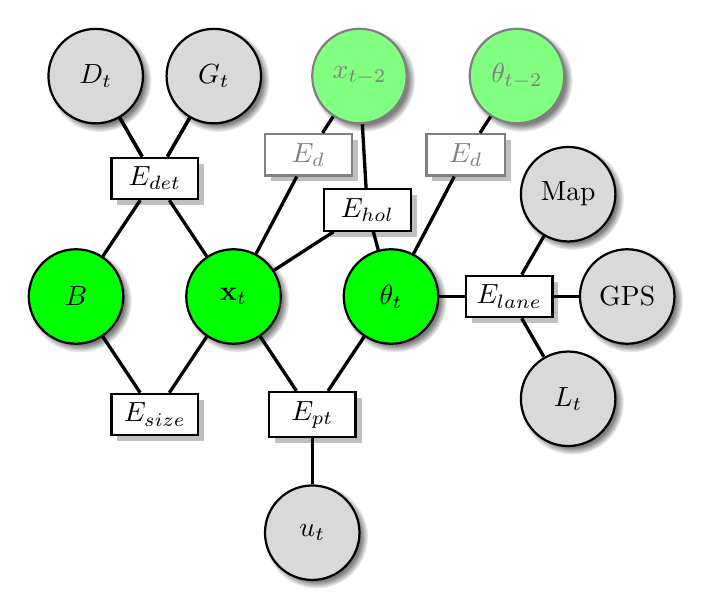
\begin{tikzpicture}[grow cyclic,line width=1.2pt,
variablenode/.style={circle,circular drop shadow,draw=black,fill=green,thick,minimum width=1.2cm},
  	  factor/.style={rectangle,drop shadow,draw=black,fill=white,thick,minimum width=1.1cm},
      obs/.style={fill=gray!30},
      prev/.style={text=gray,draw=gray,fill=green!50}]
  	  \path 

(0.6,2.8) node [variablenode,prev] (xt1) {$x_{t-2}$}
(2.6,2.8) node [variablenode,prev] (theta1) {$\theta_{t-2}$}

(-0.05,1.8) node [factor,draw=gray,text=gray] (fdynx) {$E_{d}$}
(1.95,1.8) node [factor,draw=gray,text=gray,minimum width=1cm] (fdynt) {$E_{d}$}

(.7,1.1) node[factor](fhol) {$E_{hol}$}

  	 (1, 0)  node[variablenode](theta){$\theta_t$}
   [counterclockwise from=-60,sibling angle=60]
     (2.5, 0) node [factor] (flane) {$E_{lane}$} 
    child { node [variablenode,obs] (l) { $L_t$ } }
    child { node [ variablenode,obs] (gps) {GPS}}
    child { node [ variablenode,obs] (gps) {Map}}
  	(-1, 0)  node[variablenode](xt){$\mathbf{x}_t$}

    [counterclockwise from=60,sibling angle=60]
  	(-2, 1.5) node[factor](fdet){$E_{det}$} 
  	           child {
  	             node[variablenode,obs](gp){$G_t$} 
  	  			}
	  	   		child {           node[variablenode,obs](Det){$D_t$}
  			  }

      (-2.0,-1.5) node[factor](fsize){$E_{size}$}
     (-3,0) node[variablenode](dim){$B$}
[counterclockwise from=-90]
 (0, -1.5) node[factor](fpt) {$E_{pt}$}
 child { node[variablenode,obs](pt){$u_t$} }


  	  ;
  	  \draw (xt) -- (fdet) -- (Det);
  	  \draw (xt) edge (fpt);
      \draw (fpt) -- (pt);
  	  \path  (fpt) edge (theta);
  	  \draw (fdet) -- (gp);
      \draw (fhol) -- (xt);
      \draw (fhol) -- (xt1);
      \draw (fhol) -- (theta);  	  
      \draw (dim) -- (fdet);
     \draw (xt) -- (fsize) -- (dim);
   \draw (theta) -- (flane);
   \draw (xt) -- (fdynx) -- (xt1);
   \draw (theta) -- (fdynt) -- (theta1);
	\end{tikzpicture}
